\documentclass[xcolor=dvipsnames]{beamer}
%
% Choose how your presentation looks.
%
% For more themes, color themes and font themes, see:
% http://deic.uab.es/~iblanes/beamer_gallery/index_by_theme.html
%
\mode<presentation>
{
  \usetheme{Darmstadt}      % or try Darmstadt, Madrid, Warsaw, ...
  \usecolortheme{wolverine} % or try albatross, beaver, crane, ...
  \usefonttheme{structurebold}  % or try serif, structurebold, ...
  \setbeamertemplate{navigation symbols}{}
  \setbeamertemplate{caption}[numbered]
  % eigenen stuff definieren
    % auf dieser website stehen weiter elemente von denen die farbe geändert werden kann
    % http://www.cpt.univ-mrs.fr/~masson/latex/Beamer-appearance-cheat-sheet.pdf
    % einfach ausprobieren was passt
    \definecolor{Grau}{HTML}{CCCCCC}
    \definecolor{GrauDark}{HTML}{777777} % auf weißem hintergrund
    \definecolor{Orange}{HTML}{EA5B10}
    \setbeamercolor{palette primary}{bg=Grau}
    \setbeamercolor{palette primary}{fg=BurntOrange}
    \setbeamercolor{normal text}{fg=GrauDark}
    \setbeamercolor{structure}{fg=BurntOrange} % farbe der items
    \setbeamertemplate{itemize item}[circle]
    \setbeamercolor{mini frame}{fg=BurntOrange}
    \setbeamercolor{section in head/foot}{bg=Grau}
    \setbeamercolor{section in head/foot}{fg=BurntOrange}
    \setbeamercolor{subsection in head/foot}{bg=white}
    \setbeamercolor{subsection in head/foot}{fg=GrauDark}
    \setbeamercolor{headline}{bg=Grau}
    \setbeamercolor{block body}{bg=white}
    
} 

\usepackage[utf8]{inputenc}
\usepackage[T1]{fontenc}
\usepackage{ae}
\usepackage{ngerman}
\usepackage{calc}
\usepackage{graphicx}

\title[Team 2 - Pflichtenheft]{CS:Select Pflichtenheft - Team 2}
\author{Luca Springer, Alexander Linder, Julian Dinh, Nicholas Bieker,\\ Bendix Sonnenberg}
\date{28.11.2018}

\begin{document}

\begin{frame} % das ist eine slide
  \titlepage
\end{frame}
\section{Problemstellung}
\section{Grobbeschreibung}
\section{Technische Grundlagen}
\subsection{Architektur}
\begin{frame}
\center
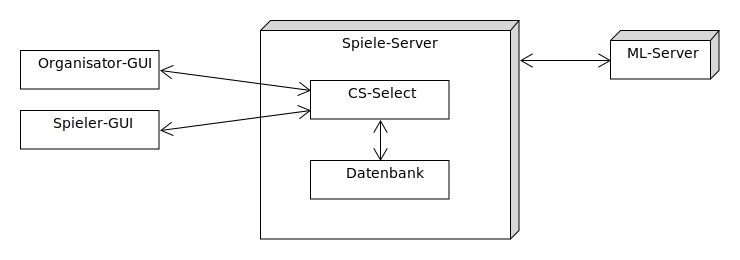
\includegraphics[width=(\textwidth) - 2cm]{../uml/export/Architektur.png}
\end{frame}
\subsection{Spiel-Server}
\begin{frame}
\begin{columns}
\begin{column}{0.5\textwidth}
         \begin{block}{CS-Select}
                \center
                \includegraphics[width=(\textwidth) / 2]{img/java.png}
                \includegraphics[width=(\textwidth) / 2]{img/tomcat.png}
                Tomcat
            \end{block} 
\end{column}
\begin{column}{0.5\textwidth}  %%<--- here
        \begin{block}{Datenbank}
                \includegraphics[width=\textwidth]{img/MySQL.jpg}
    \end{block}
\end{column}
\end{columns}
\end{frame}
\subsection{GUI}
\begin{frame}
        \includegraphics[width=5cm]{img/vue.png}
        \begin{block}{Interface}
        Vue.js Framework
        \end{block}
\end{frame}
\subsection{optional}
\begin{frame}
         \includegraphics[width=5cm]{img/docker.jpg}
         \begin{block}{Optional}
          Produkt als Docker Container liefern.
        \end{block}
\end{frame}
\section{Testfallszenarien}
    \subsection{Organisator-Testkette}
    \begin{frame}
        \begin{block} {Anmeldung, Spielerstellung}
            Der Organisator möchte sich auf dem Spiele-Server anmelden und ein neues Spiel erstellen.
        \end{block}
        \includegraphics[width=8cm]{../../pictures/Anmeldung.jpg}
    \end{frame}
    \begin{frame}
        \includegraphics[width=\textwidth]{img/Organisator_Übersicht_pres.jpg}
    \end{frame}
    \begin{frame}
         \includegraphics[width=\textwidth]{../../pictures/Spielerstellung.jpg}
    \end{frame}
    \begin{frame}
        \begin{block} {Spieler nachträglich einladen, Spiel beenden}
            Nun wird der Organisator einen neuen Spieler zum eben erstellten Spiel einladen und ein anderes aktives Spiel beenden.
        \end{block}
        \includegraphics[width=8cm]{../../pictures/2_Organisator.jpg}
    \end{frame}
    \subsection{Spieler-Testkette}
\end{document}
